\documentclass{article}

\usepackage{graphicx}
\usepackage{tikz}
\usepackage{tikzsymbols}
\usetikzlibrary{calc,patterns,shapes.geometric}
\pagestyle{empty}
\usepackage[margin=0pt]{geometry}
\geometry{papersize={14in,12in}}

\def\centerarc[#1](#2)(#3:#4:#5){\draw[#1] ($(#2)+({#5*cos(#3)},{#5*sin(#3)})$) arc (#3:#4:#5);}

\begin{document}
	\begin{figure}
		\centering
		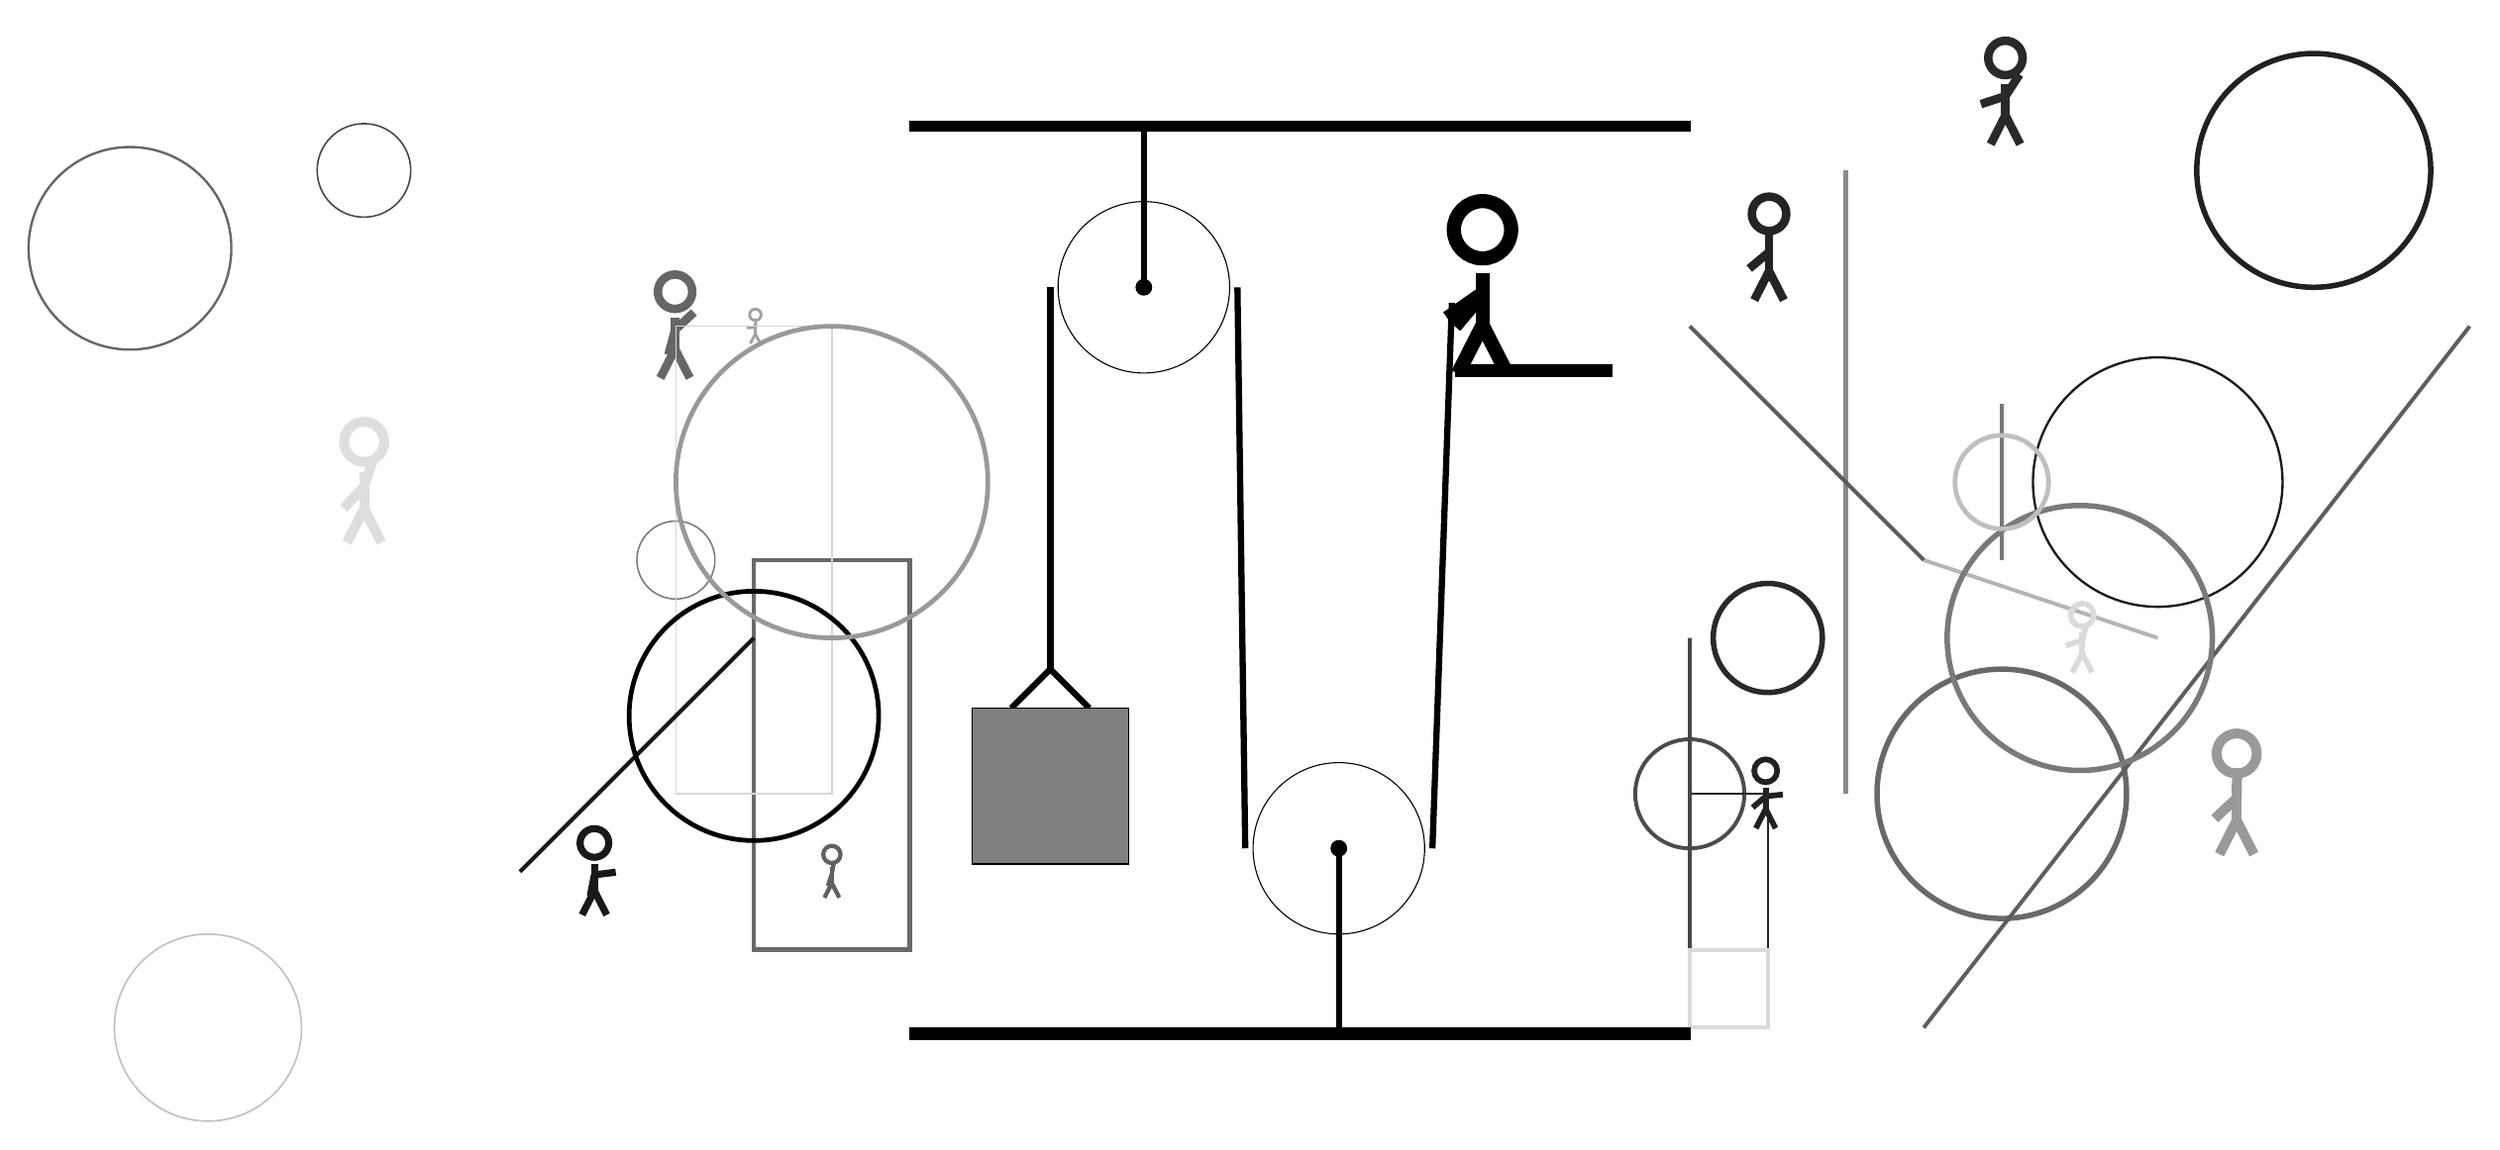
\begin{tikzpicture}
			%%%%% START %%%%%
			
			\draw[fill=black] (-2, 11.5) rectangle (8, 11.625);
			
			\draw (3.5, 2.3) circle (1.1);
			\draw[fill=black] (3.5, 2.3) circle (0.1);
			\draw[line width=0.8mm] (3.5, 2.3) -- (3.5, 0);
			
			\node[line width=0.6mm, color=black!13] at (-9, 7) {\Strichmaxerl[7][47][72]};
			
			\draw [line width=0.7mm, color=black!59](12, 3) circle (1.6);
			\node[line width=0.5mm, color=black!90] at (-6, 2) {\Strichmaxerl[5][79][7]};
			\draw [line width=0.7mm, color=black!87](16, 11) circle (1.5);
			\draw[line width=0.7mm, color=black!46] (10, 3) rectangle (10, 11);
			\draw [line width=0.2mm, color=black!25](-11, 0) circle (1.2);
			\draw [line width=0.2mm, color=black!52](-5, 6) circle (0.5);
			
			\node[line width=0.5mm, color=black!60] at (-5, 9) {\Strichmaxerl[6][75][43]};
			\node[line width=0.3mm, color=black!37] at (-4, 9) {\Strichmaxerl[2][2][85]};
			
			\draw [line width=0.5mm, color=black!70](8, 3) circle (0.7);
			\draw[line width=0.5mm, color=black!63](11, 0) -- (18, 9);
			
			\draw[line width=0.6mm, color=black!59] (-2, 1) rectangle (-4, 6);
			\draw[line width=0.5mm, color=black!29](11, 6) -- (14, 5);
			
			\node[line width=0.7mm, color=black!86] at (9, 10) {\Strichmaxerl[6][40][90]};
			\draw[line width=0.3mm, color=black!85] (8, 3) rectangle (9, 0);
			\draw [line width=0.3mm, color=black!89](14, 7) circle (1.6);
			\node[line width=0.6mm, color=black!87] at (9, 3) {\Strichmaxerl[4][41][6]};
			\draw [line width=0.3mm, color=black!60](-12, 10) circle (1.3);
			\draw [line width=0.7mm, color=black!52](13, 5) circle (1.7);
			
			\draw[line width=0.5mm, color=black!64](8, 9) -- (11, 6);
			\draw[line width=0.4mm, color=black!72] (8, 1) rectangle (8, 5);
			
			\draw[line width=0.5mm, color=black!53](12, 6) -- (12, 8);
			\node[line width=0.5mm, color=black!40] at (15, 3) {\Strichmaxerl[7][43][89]};
			\draw[line width=0.2mm, color=black!16] (-3, 9) rectangle (-5, 3);
			\draw [line width=0.6mm, color=black!25](12, 7) circle (0.6);
			
			\draw [line width=0.7mm, color=black!84](9, 5) circle (0.7);
			\draw[line width=0.5mm, color=black!91](-4, 5) -- (-7, 2);
			\draw [line width=0.6mm, color=black!100](-4, 4) circle (1.6);
			\node[line width=0.3mm, color=black!62] at (-3, 2) {\Strichmaxerl[3][72][80]};
			\draw[line width=0.5mm, color=black!15] (9, 1) rectangle (8, 0);
			\node[line width=0.4mm, color=black!84] at (12, 12) {\Strichmaxerl[6][18][57]};
			\draw [line width=0.2mm, color=black!72](-9, 11) circle (0.6);
			\draw [line width=0.6mm, color=black!40](-3, 7) circle (2.0);
			\node[line width=0.5mm, color=black!14] at (13, 5) {\Strichmaxerl[4][17][75]};
			
			\draw (1, 9.5) circle (1.1);
			\draw[fill=black] (1, 9.5) circle (0.1);
			\draw[line width=0.8mm] (1, 11.5) -- (1, 9.5);
			
			\draw[line width=0.8mm](-0.7, 4.1) --  (-0.2, 4.6) -- (0.3, 4.1);
			\draw[fill=black!50] (-1.2, 4.1) rectangle (0.8, 2.1);
			
			\draw[line width=0.8mm](-0.2, 9.5) -- (-0.2, 4.6);
			\centerarc[line width=0.8mm](1, 9.5)(180:0:1.2000000000000002)
			\draw[line width=0.8mm](2.2, 9.5) -- (2.3, 2.3);
			\centerarc[line width=0.8mm](3.5, 2.3)(180:360:1.2000000000000002)
			\draw[line width=0.8mm](4.7, 2.3) -- (4.95, 9.3);
			
			\node at (5.3, 9.5) {\Strichmaxerl[10][35][-130]};
			\draw[fill=black] (5, 8.5) rectangle (7, 8.35);
			
			\draw[fill=black] (-2, 0) rectangle (8, -0.15);
			
			%%%%% END %%%%%
		\end{tikzpicture}
	\end{figure}	
\end{document}